% Második előadás

\chapter{HEDT processzorok fejlődése}

\section{Bevezetés}

A HEDT (High-End Desktop) processzorok a nagyteljesítményű asztali gépek processzorait jelentik.
Ilyenek az Intel i7 és i9 Extreme Edition modellei.
Döntően a játékosok és tartalom kreátorok igényeit igyekeznek kiszolgálni.
Ezeknek a felhasználóknak nagy teljesítményre és jó minőségű grafikára van szükségük, ezért az ilyen processzoroknak több, akár 4 grafikus kártyát is támogatniuk kell.

\section{PCIe vonalak}
Ehhez több PCIe vonalra van szükség (kártyánként 8 vagy 16).
A Core 2 Extreme (2006 körül) család (4x8) 32 PCIe vonalpárt tartalmazott, amik az északi hídra csatlakoztak.
Ez csak a Sandy Bridge-el változott meg, ahol már a lapkára csatlakoztak.
Az Ivy Bridge előtt a PCIe 2.0 változatát támogatták a processzorok, Ivy Bridge-től pedig 3.0-t.

\section{Magszámok}
Mivel ezek a feladatok (pixelek feldolgozása) jól párhuzamosíthatók, több mag és így több memória csatorna van a HEDT processzorokban.
A magoknak csak a technológiai korlátok szabtak határt.
Kezdetben (Core 2 Extreme) ez 2 magot jelentett, majd fokozatosan 18 magra nőtt.

\begin{figure}[H]
    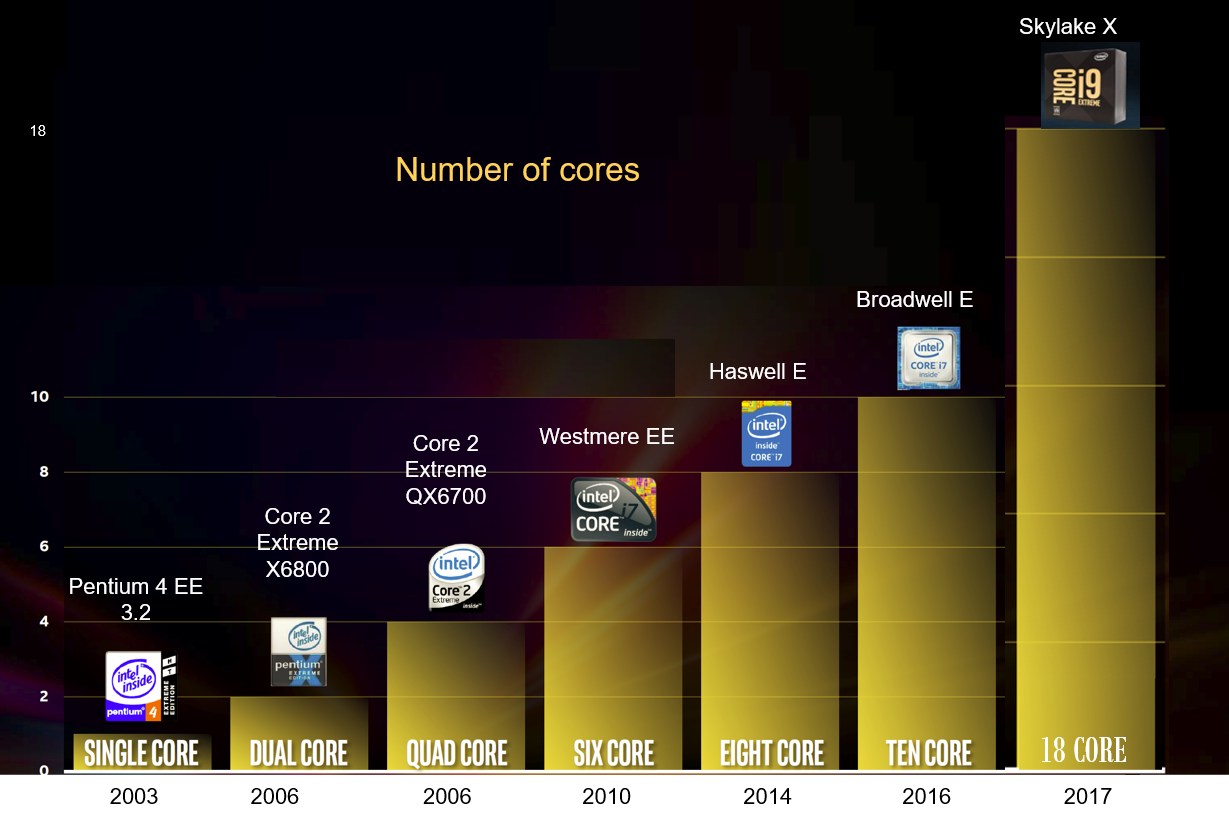
\includegraphics[width=0.8\textwidth]{cores}
    \centering
    \caption{Intel HEDT processzorok magszámának fejlődése}
    \label{fig:cores}
\end{figure}

\section{Memóriacsatornák}
A kezdetekben a viszonylag kevés mag könnyen kiszolgálható volt 2 memóriacsatornával, de ahogy növekedtek a magok számai, úgy nőtt a memóriacsatornák száma is, először 3-ra, majd 4-re.

\section{Overclocking}
A processzorok órajelét egy szorzó állítja elő, ami megszorozza a buszfrekvenciát (100/133 MHz) egy olyan faktorral, amit a Power Control Unit ad (pl. 20).
A HEDT processzorok szorzója nem rögzített, tehát a hozzáértő felhasználók növelni tudják a processzor sebességét, nagyobb disszipáció árán.

\section{Fogyasztás}
A HEDT processzorok nagy fogyasztással rendelkeznek a sok mag és memóriacsatorna miatt (130-160 W).
A processzorok teljesítményét TDP-ben szokás megadni (Thermal Design Power).
A hűtési rendszert erre az értékre kell tervezni.

\section{Grafika}
A HEDT processzorok nem tartalmaznak integrált grafikát, mivel az ilyen PC-kben jellemzően nagy teljesítményű, diszkrét grafikus kártyák dolgoznak.

